\chapter{Marco teórico} % Main chapter title

\label{ch:MarcoTeorico} % For referencing the chapter elsewhere, use \ref{Chapter1} 

%----------------------------------------------------------------------------------------


La Web contiene una gran cantidad de opiniones respecto a productos, políticos, y mucho mas, expresado en forma de noticias, sitios de opinión, reseñas en tiendas online, redes sociales. Como resultado, el problema de ``Minería de opinión'' ha obtenido una atención creciente en las ultimas dos décadas y es un factor decisivo para las nuevas organizaciones (como es mencionado en \cite{Popescu2007}). De esto mismo partimos que el análisis de textos para extraer el significado y demás componentes extraíbles del texto componen un factor que debe considerarse al momento de realizar decisiones, de manera que los avances hechos hasta ahora tienen como meta una aplicación practica de lo que se conoce como \glsentrylong{nlp}.

Luego de los ataques terroristas del 11 de Septiembre de 2001 en Estados Unidos, se realizaron fuertes criticas respecto a la inteligencia, donde el director del FBI~\emph{Robert~S.~Mueller} indico que el principal problema que la agencia tuvo fue que se enfocaba demasiado en lidiar con el crimen luego de que fue cometido y ponía muy poco énfasis en prevenirlo (adaptado de \cite{mena2003investigative}). Es por esto que el uso de \gls{nlp} para temas de seguridad como también de metodologías de \glsentrylong{machinel} y \glsentrylong{deepl} han sido ampliamente utilizadas en ámbito de seguridad luego de estos eventos.

Para obtener una mejor inteligencia se necesito de mejores tecnologías a las que se tenían entonces (véase \cite[p\'ag 2]{mena2003investigative}):
\begin{itemize}
\item Integración de datos (\'o \gls{dataintegration} en ingl\'es)
\item Análisis de vínculos (\'o \gls{linkanalisys} en ingl\'es)
\item Agentes de software (\'o \gls{softwareagents} en ingl\'es)
\item Minería de texto (\'o \gls{textmining} en ingl\'es)
\item Redes neuronales (\'o \gls{neuralnetwork} en ingl\'es)
\item Algoritmos de \glsentrylong{machinel} (\'o \gls{mlalgorithms} en ingl\'es)
\end{itemize}

% ================================================================

\section{Análisis de vínculos (\glsentrylong{linkanalisys})}
Es la visualización de asociaciones entre entidades y eventos, por lo general involucran una visualización por medio de una gráfica o un mapa que muestre las relaciones entre sospechosos y ubicaciones, sea por medio físico o por comunicaciones en la red.

% ================================================================

\section{Agentes de software (\glsentrylong{softwareagents})}
Es el software que realiza tareas asignadas por el usuario de manera autónoma, donde sus habilidades básicas son:
\begin{itemize}
\item \textbf{Realización de tareas:} Hacen obtención de información, filtrado, monitoreo y reporte.
\item \textbf{Conocimiento:} Pueden usar reglas programadas, o pueden aprender reglas nuevas (véase \ref{sec:KBS}).
\item \textbf{Habilidades de comunicación:} Reportar a humanos e interactuar con otros agentes.
\end{itemize}

% ================================================================

\section{Aprendizaje de maquina (\glsentrylong{machinel})} \label{sec:ML}
De acuerdo con \cite{murphymachinel}, se define como un conjunto de métodos que pueden detectar patrones automáticamente en datos, y luego usar los patrones descubiertos para predecir los datos futuros, o realizar otra clase de toma de decisiones con un grado de incertidumbre, por tal motivo es necesario el uso de teoría de probabilidad, que puede ser aplicada a cualquier tipo de problema que involucra incertidumbre.

\subsection{Tipos de \glsentrylong{machinel}}
\gls{machinel} esta principalmente dividida en dos tipos. El método predictivo o bien \textbf{aprendizaje supervisado} (\gls{supervisedl}), donde el objetivo es aprender un mapeo de las entradas $\mathbf{x}$ a las salidas $y$, dado un conjunto de pares de etiquetas de entrada--salida $D = \{(\mathbf{x}_i, y_i)\}_{i=1}^{N}$. $D$ se le llama el conjunto de entrenamiento y $N$ es el numero de muestras de entrenamiento.

En la forma mas sencilla, cada entrada de entrenamiento $\mathbf{x}_i$ es un vector $D$--dimensional de números, a estos se le llaman \emph{características} o \emph{atributos}.

De manera similar la forma de la salida puede ser en principio cualquier cosa, pero la mayoría de métodos asumen que $y_i$ es una variable \emph{categórica} o \emph{nominal} de algún conjunto finito, $y_i \in \{1,\ldots,C\}$, o que $y_i$ es un escalar real, $y_i \in \mathbb{R}$. Cuando la variable $y_i$ es categórica, al problema se le reconoce como \textbf{clasificación} o \textbf{reconocimiento de patrones}, y cuando es un valor real se le conoce como un problema de \textbf{regresión}.

El segundo tipo principal de \gls{machinel} es el descriptivo o \textbf{aprendizaje no--supervisado} (\gls{unsupervisedl}), en este solo están disponibles los datos de entrada $D = \{\mathbf{x}_i\}_{i=1}^{N}$, y la meta es encontrar ``patrones interesantes'' en los datos. Este es un problema mucho menos definido, debido a que no se conocen los tipos de patrones que se quieren encontrar, y no hay una métrica obvia de error (no como aprendizaje supervisado en la que se puede comparar nuestra predicción de $y$ para un $\mathbf{x}$ con el valor observado).

Un tercer tipo de aprendizaje de maquina es conocido como \textbf{\gls{reinforcedl}}, el cual es un tipo menos usado. Este es útil cuando se quiere aprender como actuar o comportarse cuando se recibe una recompensa ocasional o una señal de castigo.

\subsection{Sistemas de Detección de Anomalías (\glsentrylong{anomalydetectionsys})}
\todo{Pendiente}


% ================================================================
\section{Mineria de datos (\glsentrylong{datamining})} \label{sec:datamining}
Según \cite{tan2005introduction}, la minería de datos se define como el proceso de descubrir información útil en repositorios grandes de datos. Las técnicas de minería de datos son desplegadas para limpiar grandes bases de datos para encontrar patrones nuevos y útiles que de lo contrario podrían permanecer desconocidos. También ofrecen capacidades para predecir la salida de observaciones futuras, tales como predecir si un cliente nuevo gastara mas de \$100 en una tienda.

No todas las tareas de descubrimiento de información son considerados como \gls{datamining}. Por ejemplo, realizar una consulta de campos individuales usando un sistema de base de datos o encontrar una pagina web por medio de una búsqueda en Internet son tareas relacionadas con \emph{adquisición de información}.

\subsection{Mineria de texto (\glsentrylong{textmining})} \label{subsec:NLP}
Es un subcampo de Inteligencia Artificial conocida como \glsentrylong{nlp}, en donde las herramientas de minería de datos pueden capturar rasgos críticos del contenido de un documento basado en el análisis de sus características lingüísticas.

La mayoría de los crímenes son electrónicos por naturaleza, por lo que se dejan rastros textuales que investigadores pueden seguir y analizar. Estas se enfocan en el descubrimiento de relaciones en texto no--estructurado y pueden ser aplicados al problema de \emph{búsqueda} y \emph{localización de palabras clave}.

\subsection{Clasificación} \label{subsec:clasification}
Clasificación es la tarea de asignarle una de varias categorías predefinidas a objetos, y es una tarea que tiene una variedad extensa de aplicaciones. Ejemplos de esto se encuentran la detección de correos no deseados en mensajes de e--mails basándose del encabezado o el cuerpo del mensaje, categorización de células benignas de malignas basándose en los resultados de escaneados MRI o incluso la clasificación de galaxias basado en su forma.

Definido formalmente, clasificación es la tarea de aprender una función objetivo $f$ que mapea cada conjunto de atributos $x$ a una clase predefinida de etiquetas $y$.

La función objetivo también se define informalmente como un \emph{modelo de clasificación}.

\subsubsection{Metodologías de clasificación} \label{subsubsec:classmethods}
Existen muchos métodos para la clasificación de datos no--estructurados, entre los descritos aquí están:
\begin{itemize}
\item Clasificador basado en reglas (véase \ref{sec:KBS})
\item Redes neuronales artificiales (véase \ref{sec:ANN})
\item Maquinas de soporte vectorial (véase \ref{sec:SVM})
\item Clasificador de Na\"{\i}ve Bayes (véase \ref{subsec:naivebayes})
\end{itemize}

\subsection{Clustering} \label{subsec:clustering}
El análisis de clusters agrupa objetos de datos basándose únicamente en la información encontrada en los datos que describen los objetos y sus relaciones. El objetivo es que objetos dentro de un grupo sean similares (o relacionados) el uno al otro, y que sean diferentes (o sin relación) a objetos en otros grupos. Entre mayor sea la similitud dentro de un grupo y entre mayor sea la diferencia entre grupos, sera mejor o mas distintivo el clustering.

Los métodos de clustering se hacen referencia comúnmente en \gls{machinel} como métodos no--supervisados, los cuales se describen en \ref{sec:ML}. Un método de estos se describe en \ref{subsec:SOM} conocidos como mapas autoorganizados.

% ================================================================

\section{Sistemas Basados en Conocimiento (\glsentrylong{kbs})} \label{sec:KBS}
Según \cite{sajja2010knowledge}, los \gls{kbs} son uno de los mayores miembros de la familia de \gls{ai}. El \gls{kbs} consiste de una \gls{knowledgebase} y un programa de búsqueda llamado \gls{inferenceengine} representado en la \figureref{fig:kbs-arch}. La \gls{knowledgebase} puede ser usado como un repositorio de conocimiento de varias formas.

Existen 5 tipos de \gls{kbs}, donde uno de ellos es conocido como \gls{expertsystems}, usados como \gls{rulebasedsys}, donde su \gls{knowledgebase} esta dado como reglas y el \gls{inferenceengine} esta dado por algo llamado \gls{workingmemory}, que representa los hechos que se conocen inicialmente del sistema junto con los hechos que se van dando como inferencia de las reglas.

\begin{figure}[H]
\centering
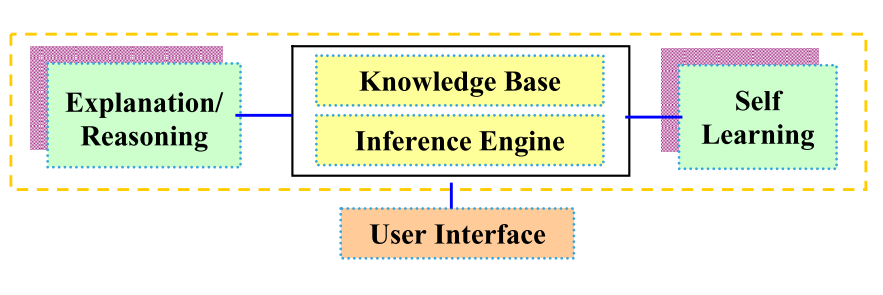
\includegraphics[scale=0.4]{Figures/kbs-architecture.png}
\decoRule
\caption[Arquitectura \glsentrytext{kbs}]{Arquitectura \glsentrytext{kbs}. Tomado de \cite{sajja2010knowledge}}
\label{fig:kbs-arch}
\end{figure}

Estas reglas pueden resumirse como una colección de condicionales de la forma \textbf{IF/ELSE} que se componen de un \emph{antecedente} y un \emph{consecuente}.

Existen dos tipos de \gls{rulebasedsys}, definidos como \gls{deductivesys} y \gls{reactivesys}, donde el \gls{deductivesys} tiene como objetivo realizar una conclusión en base a los hechos iniciales en la \gls{workingmemory}, por el otro lado se tienen los \gls{reactivesys}, los cuales de igual manera a los \gls{deductivesys}, toman los hechos de la \gls{workingmemory} y realizan sea una acción interactiva con su entorno o bien una modificación de los hechos que se encuentran en la \gls{workingmemory} tal como la adición o eliminación de hechos. Tómese el ejemplo de la \equationref{eq:rbs-example} tomada de \cite{Mendel}, donde \emph{x} es la temperatura y \emph{AC} es aire acondicionado.

\begin{equation} \label{eq:rbs-example}
  \left\{ \begin{array}{ll}
            \text{IF x es moderado,} & \text{THEN y = ajustar AC a bajo} \\
            \text{IF x es alto,}     & \text{THEN y = ajustar AC a moderado a alto} \\
            \text{IF x es muy alto,} & \text{THEN y = ajustar AC a alto} 
          \end{array} \right.
\end{equation}

\subsection{Fuzzy Knowledge Based Systems}
\todo{Pendiente}


% ================================================================

\section{Redes Neuronales Artificiales (\glsentrylong{neuralnetwork})} \label{sec:ANN}
El estudio de redes neuronales artificiales fue inspirado por los intentos de simular los sistemas biológicos de neuronas. El cerebro humano se compone principalmente de células nerviosas llamadas \emph{neuronas}, enlazadas con otras neuronas por medio de hebras de fibra conocidas como \emph{axones}. Los axones son usados para transmitir impulsos nerviosos de una neurona a otra cada vez que las neuronas son estimuladas. Una neurona esta conectada a axones de otras neuronas por medio de \emph{dendritas}, las cuales son extensiones desde el cuerpo de la neurona. El punto de contacto entre una dendrita y un axón se conoce como \emph{sinapsis}. Los neurólogos han descubierto que el cerebro humano aprende por medio de cambiar la fuerza de la conexión sináptica entre las neuronas a través de estimulación repetitiva por el mismo impulso.

De manera análoga a la estructura del cerebro humano, una \gls{neuralnetwork} se compone de una estructura interconectada de nodos y vínculos directos.

\subsection{Mapa autoorganizado (\glsentrylong{som})} \label{subsec:SOM}
El objetivo principal de los \gls{som} es de transformar una patrón de entrada $m$--dimensional en un mapa discreto uni-- o bi--dimensional, donde sus principales características es que es un algoritmo que se basa en \gls{unsupervisedl}, es \gls{feedforward}, tiene una sola capa de neuronas donde su propósito es realizar \gls{clustering} y una reducción de dimensionalidad sobre los datos de una forma topologicamente ordenada.

Los \gls{som} tienen tres características distintivas:
\begin{itemize}
\item {\bf Competencia:} por cada patrón de entrada, las neuronas en la red competirán entre ellas para determinar un ganador.
\item {\bf Cooperación:} la neurona ganadora determina la ubicación espacial (vecinos) alrededor de donde otras vecinas también se verán estimuladas.
\item {\bf Adaptación:} la neurona ganadora como también sus vecinas tendrán sus pesos asociados actualizados, y se tiene que los vecinos entre mas cerca estén del ganador, mayor es el grado de adaptación.
\end{itemize}

El algoritmo de aprendizaje de \gls{som} parte de primero inicializar los pesos de las $o$ neuronas con pesos aleatorios pequeños de una distribución de probabilidad aleatoria o uniforme, donde cada vector de entrada se define como $x = [x_1, \ldots, x_m]^{T} \in \mathbb{R}^{m}$ y la entrada general de $N$ patrones como $\mathbf{X}^{m \times N}$, el vector de pesos de la neurona $i$ es $\mathbf{w}_i = [w_{i1}, \ldots, w_{im}] \in \mathbb{R}^{1 \times m}$, con la matriz de pesos $\mathbf{W}^{o \times m}$.

Para alcanzar el objetivo de \emph{competencia}, se realiza por cada patrón de entrada $x_i$ una comparación con cada uno de los pesos de las $o$ neuronas y se establece la de menor distancia respecto $x_i$ (típicamente la distancia Euclidiana), dejando un ganador $winner$, tal como en la \equationref{eq:som-competition}.
\begin{equation} \label{eq:som-competition}
  winner = \text{argmin}_j \norm{x_i - w_j} ; j = 1, \ldots,o
\end{equation}

Luego de establecer la neurona ganadora, se realiza el paso para alcanzar la \emph{cooperación}, que consiste en que por medio de una función kernel $h$ (típicamente una una distribución gaussiana), que permite establecer un área de afectación de las otras neuronas según su ubicación física en el mapa, definidos como $r_{winner}$ y $r_j$ que son la ubicación de la neurona ganadora y la neurona vecina $j$, en el cual el grado de afectación de la neurona vecina depende de la distancia de la que esta de la neurona ganadora, definido en la \equationref{eq:som-cooperation}.
\begin{equation} \label{eq:som-cooperation}
  h_{j, winner}(t) = \text{exp}\Bigg(\frac{- \norm{r_j - r_{winner}}^2}{ 2 \sigma(t)^2}\Bigg)
\end{equation}

Parte importante del proceso de convergencia del \gls{som} es que a medida que avanzan las iteraciones $t$ del algoritmo el área de afectación se va reduciendo como parte del proceso de adaptación, por lo que definimos $\sigma(t) = \sigma_0 \text{exp}(-t / \tau_1)$, donde $\tau_1$ es una constante heurística y $\sigma_0$ la dimensión del mapa \gls{som}.

Finalmente para alcanzar la \emph{adaptación} se realiza una actualización de los pesos de la matriz $\mathbf{W}$ en base a la influencia de área $\sigma(t)$ y de una tasa de aprendizaje $\alpha(t) = \alpha_0 \text{exp}(-t/ \tau_2)$, donde $\tau_2$ es otra constante heurística y $\alpha_0$ es una constante de aprendizaje inicial, que debe ser $0 \le \alpha_0 \le 1$, la actualización se describe por la \equationref{eq:som-adaptation} y el proceso puede ser visto gráficamente en la \figureref{fig:som-adap-proc}, tanto de forma uni-- como bi--dimensional.
\begin{equation} \label{eq:som-adaptation}
  w_j(t+1) = w_j(t) + \alpha(t) h_{j, winner}(t)\Big[x_i-w_j(t)\Big]
\end{equation}

\begin{figure}[H]
\centering
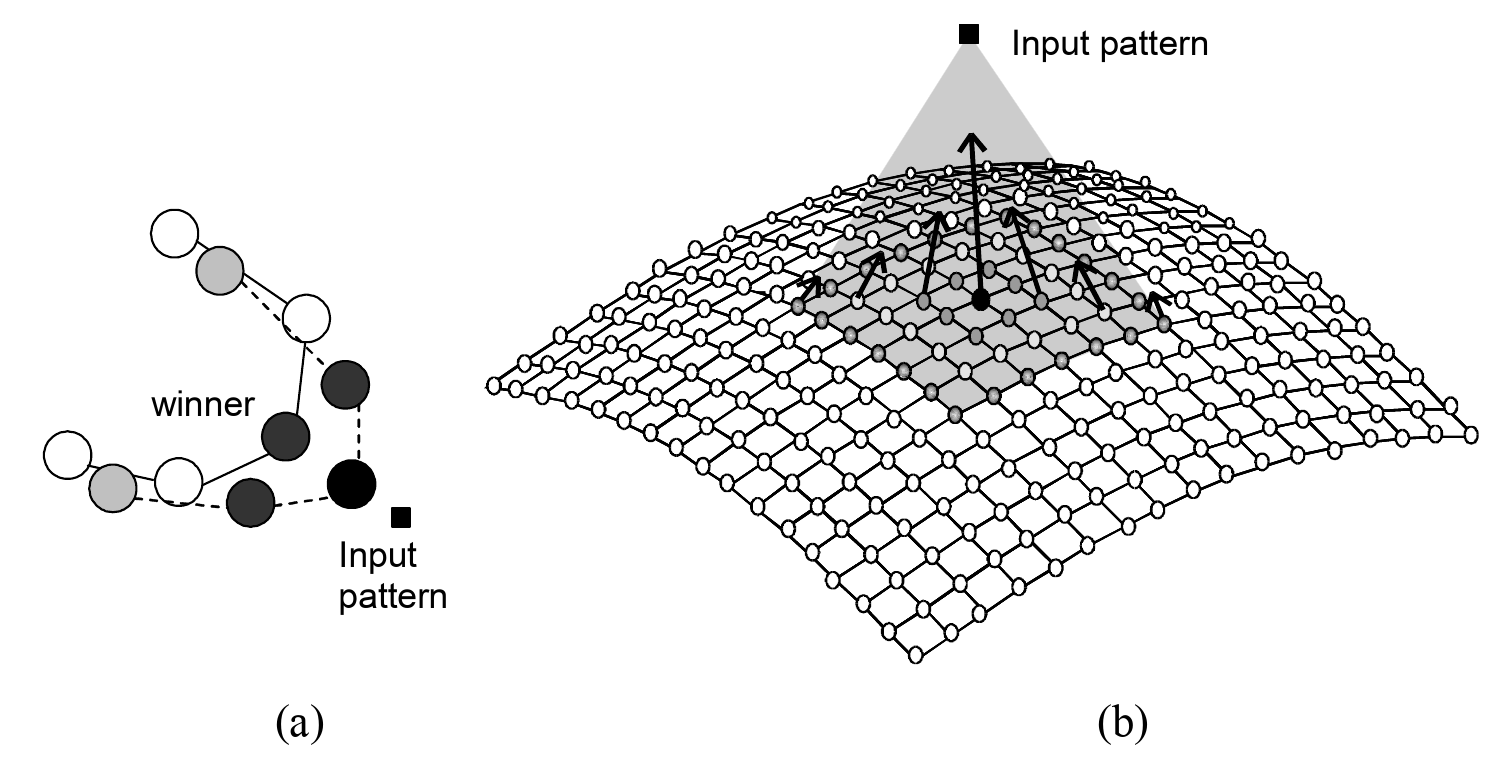
\includegraphics[scale=0.2]{Figures/som-adaptive-proc.png}
\decoRule
\caption[Proceso de adaptación de \glsentrytext{som}]{Proceso de adaptación de \glsentrytext{som}, (a) uni--dimensional, (b) bi--dimensional. Tomado de \cite{de2006fundamentals}}
\label{fig:som-adap-proc}
\end{figure}

Luego de que el algoritmo de aprendizaje termina de realizar las iteraciones, la salida de este es la matriz de pesos $\mathbf{W}$, en la \figureref{fig:som-impl-example} se puede apreciar una aproximación del algoritmo con un mapa uni--dimensional tratando de aproximar una función sinusoidal con ruido adicionado en un gráfico 2D.

\todo{agregar texto que describa la figura \ref{fig:som-example}}

\begin{figure}[H]
\centering
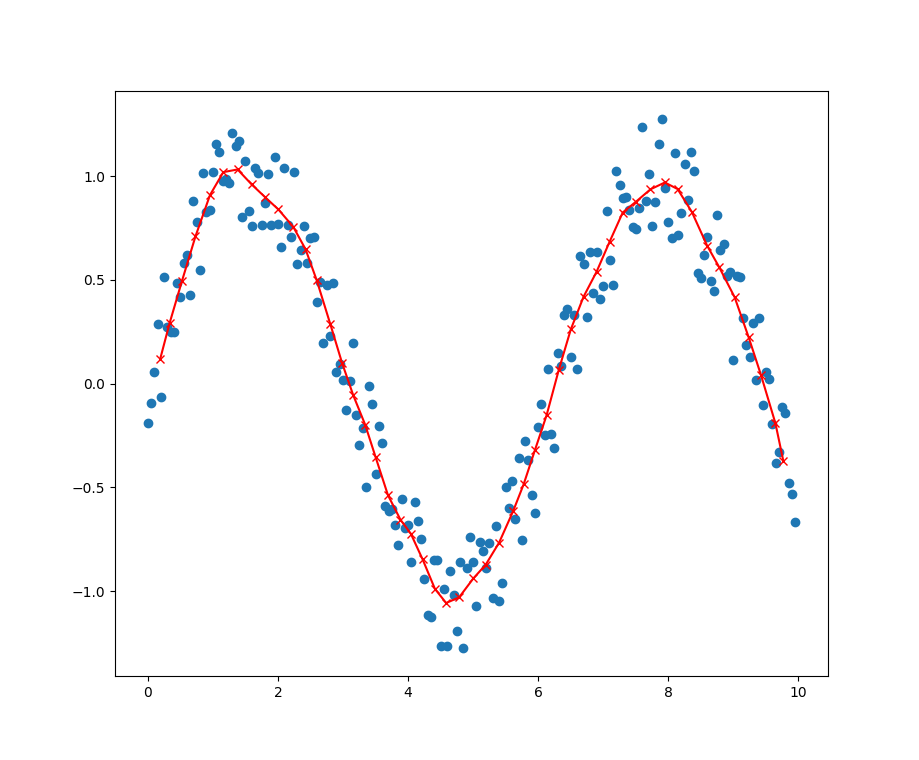
\includegraphics[scale=0.5]{Figures/som-implementation-example.png}
\decoRule
\caption[Ejemplo de salida de \glsentrytext{som} uni-dimensional]{Ejemplo de salida de \glsentrytext{som} uni-dimensional. Implementación propia.}
\label{fig:som-impl-example}
\end{figure}

\begin{figure}[H]
\centering
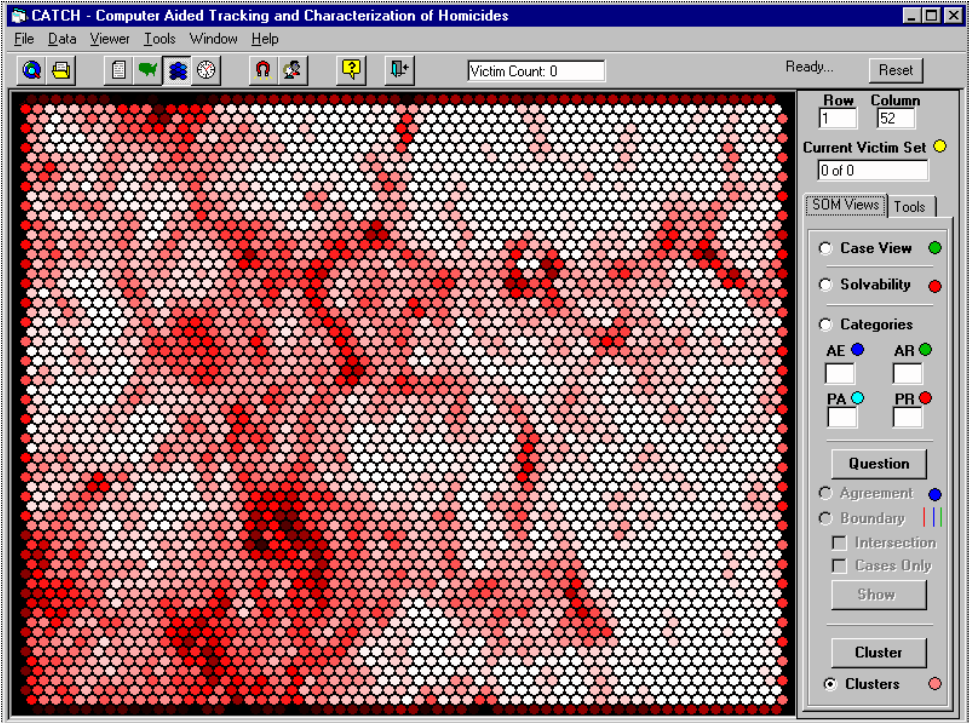
\includegraphics[scale=0.3]{Figures/som-example.png}
\decoRule
\caption[Ejemplo de uso de \glsentrytext{som} en aplicaciones de perfilado]{Ejemplo de uso de \glsentrytext{som} en aplicaciones de perfilado. Tomado de \cite{mena2003investigative}}
\label{fig:som-example}
\end{figure}

% ================================================================

\section{Maquina de soporte vectorial (\glsentrylong{svm})} \label{sec:SVM}
\gls{svm} es una técnica de clasificación que tiene sus raíces en la teoría de aprendizaje estadístico que ha mostrado resultados empíricos prometedores en muchas aplicaciones practicas, desde reconocimiento de dígitos escritos a mano a categorización de texto. \gls{svm} también funciona muy bien con datos de alta dimensionalidad. Otro aspecto destacable de esta aproximación es que representa la frontera de decisión usando un subconjunto de las muestras de entrenamiento, conocidos como los \emph{support vectors}.

\subsection{Maximum Margin Hyperplanes}
Se puede entender a los \gls{mmh} como hiper-planos que ayudan a separar datos en un hiper-espacio y que poseen un margen de decisión entre los datos, como ejemplo tómese la \figureref{fig:svm-hyperplanes}, donde el hiper-plano $B_1$ tiene un margen de decisión mas grande que el hiper-plano $B_2$.

\begin{figure}[H]
\centering
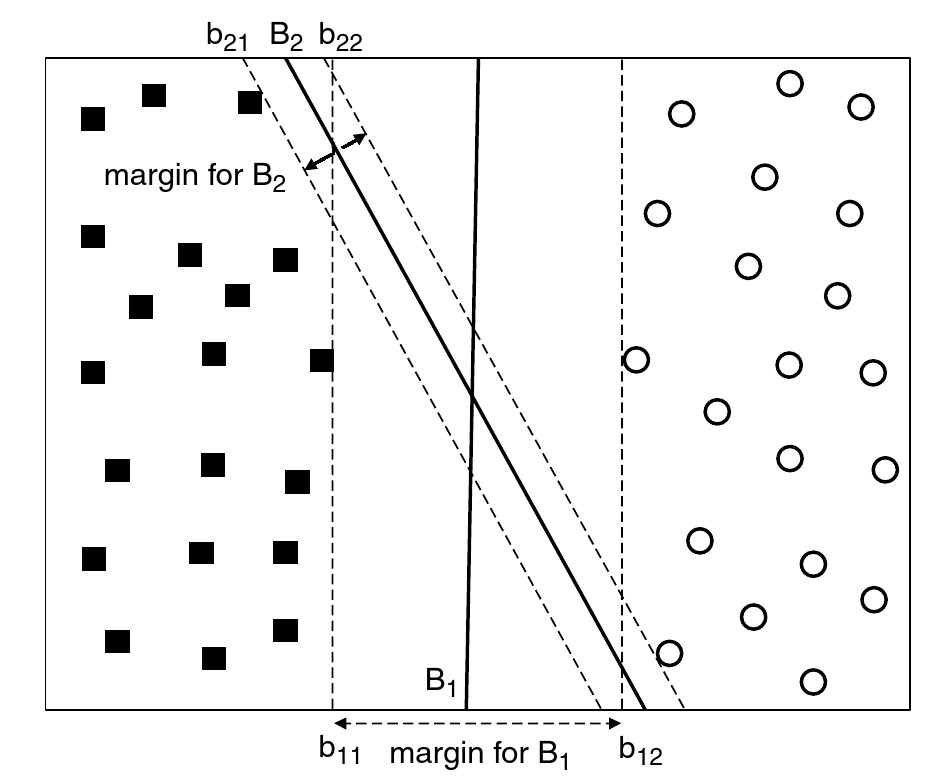
\includegraphics[scale=0.3]{Figures/svm-hyperplanes.png}
\decoRule
\caption[\glsentryname{mmh}]{\glsentryname{mmh}. Tomado de \cite{tan2005introduction}}
\label{fig:svm-hyperplanes}
\end{figure}

Finalmente, el objetivo final de los \gls{svm} es la búsqueda de un hiper-plano con el mayor margen de decisión. Existen dos tipos de \gls{svm}, el lineal y el no--lineal. El lineal realiza la separación de los datos con su hiper-plano a partir de los datos de entrada en su espacio vectorial original, mientras que el no--lineal consta de realizar una transformación de los espacios de los datos de entrada a uno en que sea linealmente separable (véase como ejemplo la \figureref{fig:svm-nonlinear-transforms}), sin embargo al realizar la transformación, el algoritmo de \gls{svm} se ve afectado por la dimensionalidad de la entrada, por lo que existe lo que se conoce como la función \emph{kernel} para remediarlo.

\begin{figure}[H]
\centering
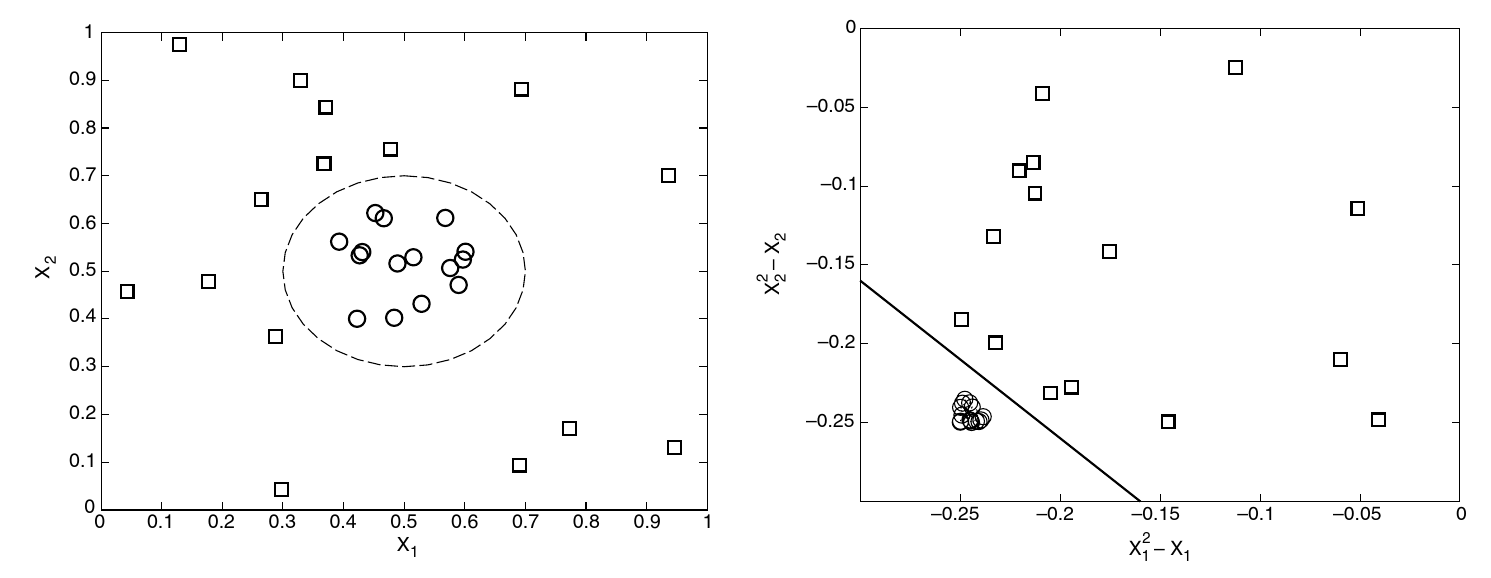
\includegraphics[scale=0.25]{Figures/svm-nonlinear-transform.png}
\decoRule
\caption[Transformación de espacios en \glsentrylong{svm}]{Transformación de espacios en \glsentrylong{svm}. Tomado de \cite{tan2005introduction}}
\label{fig:svm-nonlinear-transforms}
\end{figure}

\subsection{Función Kernel}
La función polinomial de similaridad, $K$, la cual es calculada en el espacio original de los datos de entrada, se le conoce como la \textbf{función Kernel}. En principio se asegura que la función kernel puede ser expresada siempre como el producto punto entre dos vectores de entrada en algún espacio de alta dimensionalidad, la función de kernel también tiene la particularidad de que el computo de los productos punto con la función toman considerablemente menos tiempo que realizar la transformación de espacios, dejando de lado la transformación, acelerando la tarea de clasificación.

% ================================================================

\section{Clasificadores Bayesianos} \label{sec:bayes}
En muchas aplicaciones de relaciones entre el conjunto de atributos y la etiqueta es no--determinante. Es decir, la etiqueta de clase de un dato de un conjunto de prueba no puede ser determinado con certeza a pesar de ser un atributo idéntico a los atributos de entrenamiento. Esto puede ser producto de que los datos poseen ruido o la presencia de ciertos factores que afectan la clasificación pero no son incluidos en el análisis. Para esto es crucial el teorema de Bayes, el cual es un principio estadístico que combina el conocimiento previo de las clases con la nueva evidencia que se obtiene de los datos.

\subsection{Teorema de Bayes} \label{subsec:bayestheo}
El teorema de Bayes dice que para un par de variables aleatorias $X$ y $Y$ y que $P(X=x | Y=y)$ la probabilidad de que la variable $X$ tome el valor $x$ dado que el valor de la variable $Y$ es $y$. Se tiene entonces la \equationref{eq:bayestheo}.
\begin{equation} \label{eq:bayestheo}
  P(Y | X) = \frac{P(X | Y) P(Y)}{P(X)}
\end{equation}

\subsubsection{Usando el teorema de Bayes para clasificación}
Para denotar el problema de clasificación desde una perspectiva estadística se define a $X$ como el conjunto de atributos y $Y$ como el conjunto de etiquetas de clase. Si la etiqueta de clase tiene una relación no--determinante con los atributos, entonces se pueden tomar a $X$ y a $Y$ como variables aleatorias y capturar su relación probabilística con $P(Y|X)$, conocida como la probabilidad posterior para $Y$, dada su probabilidad previa $P(Y)$.

Durante la fase de entrenamiento, es necesario aprender las probabilidades posteriores $P(Y|X)$ para cualquier combinación de $X$ y $Y$ basándose en la información recolectada de los datos de entrenamiento.

Dado que lo que se quiere realizar es una clasificación que represente la probabilidad de que dado un valor de $X=x$ este relacionado con que $Y=y$, se puede reconocer primero que $X$ se mantiene constante para lo que son los datos de entrenamiento, y que lo desconocido sea la clasificación $Y=y$ con probabilidad $P(Y|X)$, al conocer esta probabilidad, un valor de prueba $X'$ puede ser clasificado por medio de encontrar la clase $Y'$ que maximice la probabilidad posterior $P(Y'|X')$.


\subsection{Clasificador Na\"{\i}ve Bayes} \label{subsec:naivebayes}
Un clasificador de Na\"{\i}ve Bayes estima la probabilidad condicional de las clases por medio de suponer que los atributos son condicionalmente independientes, dado la etiqueta de clasificación $y$. La suposición de independencia condicional se puede dar por la \equationref{eq:bayes-conditional-independence}.

\begin{equation} \label{eq:bayes-conditional-independence}
  P(X|Y=y) = \prod_{i=1}^{d} P(X_i|Y=y)
\end{equation}

Donde cada conjunto de atributos $X=\{ X_1, \ldots, X_d \}$ que consiste de $d$ atributos.
\subsubsection{Como funciona el clasificador Na\"{\i}ve Bayes}
Con la suposición de independencia condicional, en vez de computar la probabilidad condicional de clases para cada combinación de $X$, solo se debe realizar para establecer la probabilidad condicional de cada $X_i$, dado $Y$.

Para clasificar un dato de prueba, el clasificador computa la probabilidad posterior para cada clase $Y$ como se muestra en la \equationref{eq:bayes-classifier}.

\begin{equation} \label{eq:bayes-classifier}
  P(Y|X) = \frac{P(Y) \prod_{i=1}^{d}P(X_i|Y)}{P(X)}
\end{equation}

